
\subsection{Tipanje problema}
Pričel sem z neokrnjeno, kvadratno \emph{tabulo raso}. Uveril sem se, da znam poiskati lastne nihajne načine in pripadajoče lastne vrednosti. Po pripravi matrike $A$ sem ugotovil, da metoda \texttt{scipy.linalg.eigh} deluje odlično, metode iz naprednejšega modula \texttt{scipy.sparse.linalg} pa so malenkost zahtevnejše, vendar s pravo optimizacijo parametrov povrnejo ekvivalentne rezultate.

Prvih nekaj lastnih vrednosti prikazujem spodaj. Opazimo, da lastne vrednosti ležijo druga na drugi, ker pa imajo vsake oči svojega malarja, sem preveril še numerično ekvivalenco obeh vektorjev lastnih vrednosti:
\begin{python}
np.allclose(eigenvalues_sparse[:16], eigenvalues[:16])
True
\end{python}
\begin{center}
    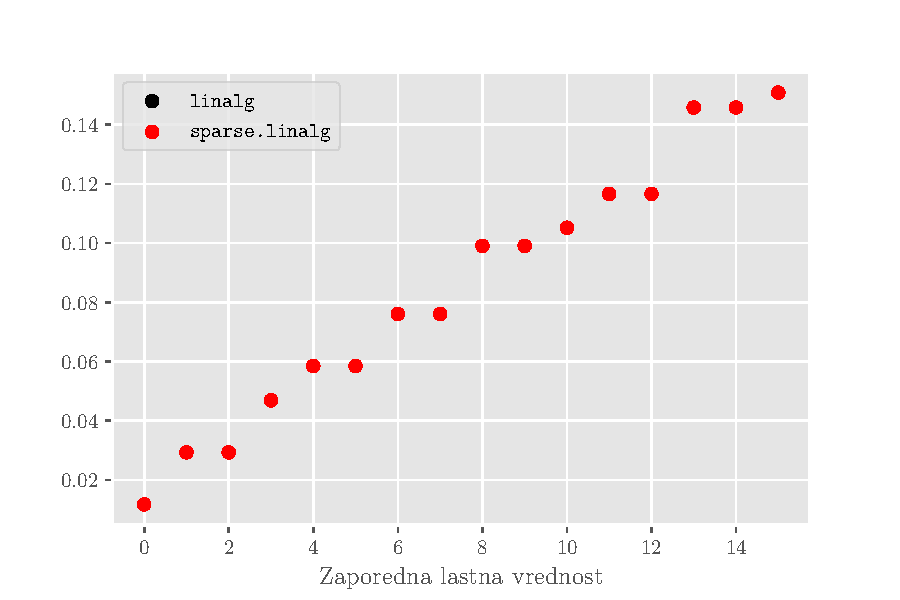
\includegraphics[width=0.7\textwidth]{../old/1-0-spekter-zoom.pdf}
\end{center}
Če nadaljujemo raziskovanje lastnih vrednosti vse do višjih, dobim ponovno ekvivalenco naračunanih lastnih vrednosti. Izgled polnega spektra prikazujem spodaj:
\begin{center}
    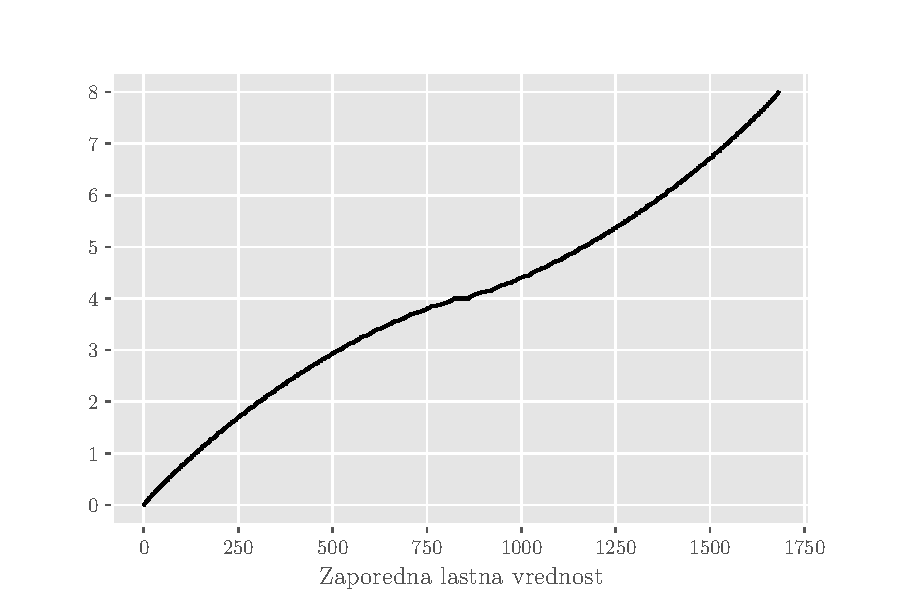
\includegraphics[width=0.7\textwidth]{../old/1-0-spekter.pdf}
\end{center}
Akademska radovednost veli, da izrišemo vsaj nekaj osnovnih nihajnih načinov,  ki jih porodita obe metodi. Za 'klasično' metodo, ki ne upošteva posebnih odlik vhodne matrike, dobim sledečo sliko.
\begin{center}
    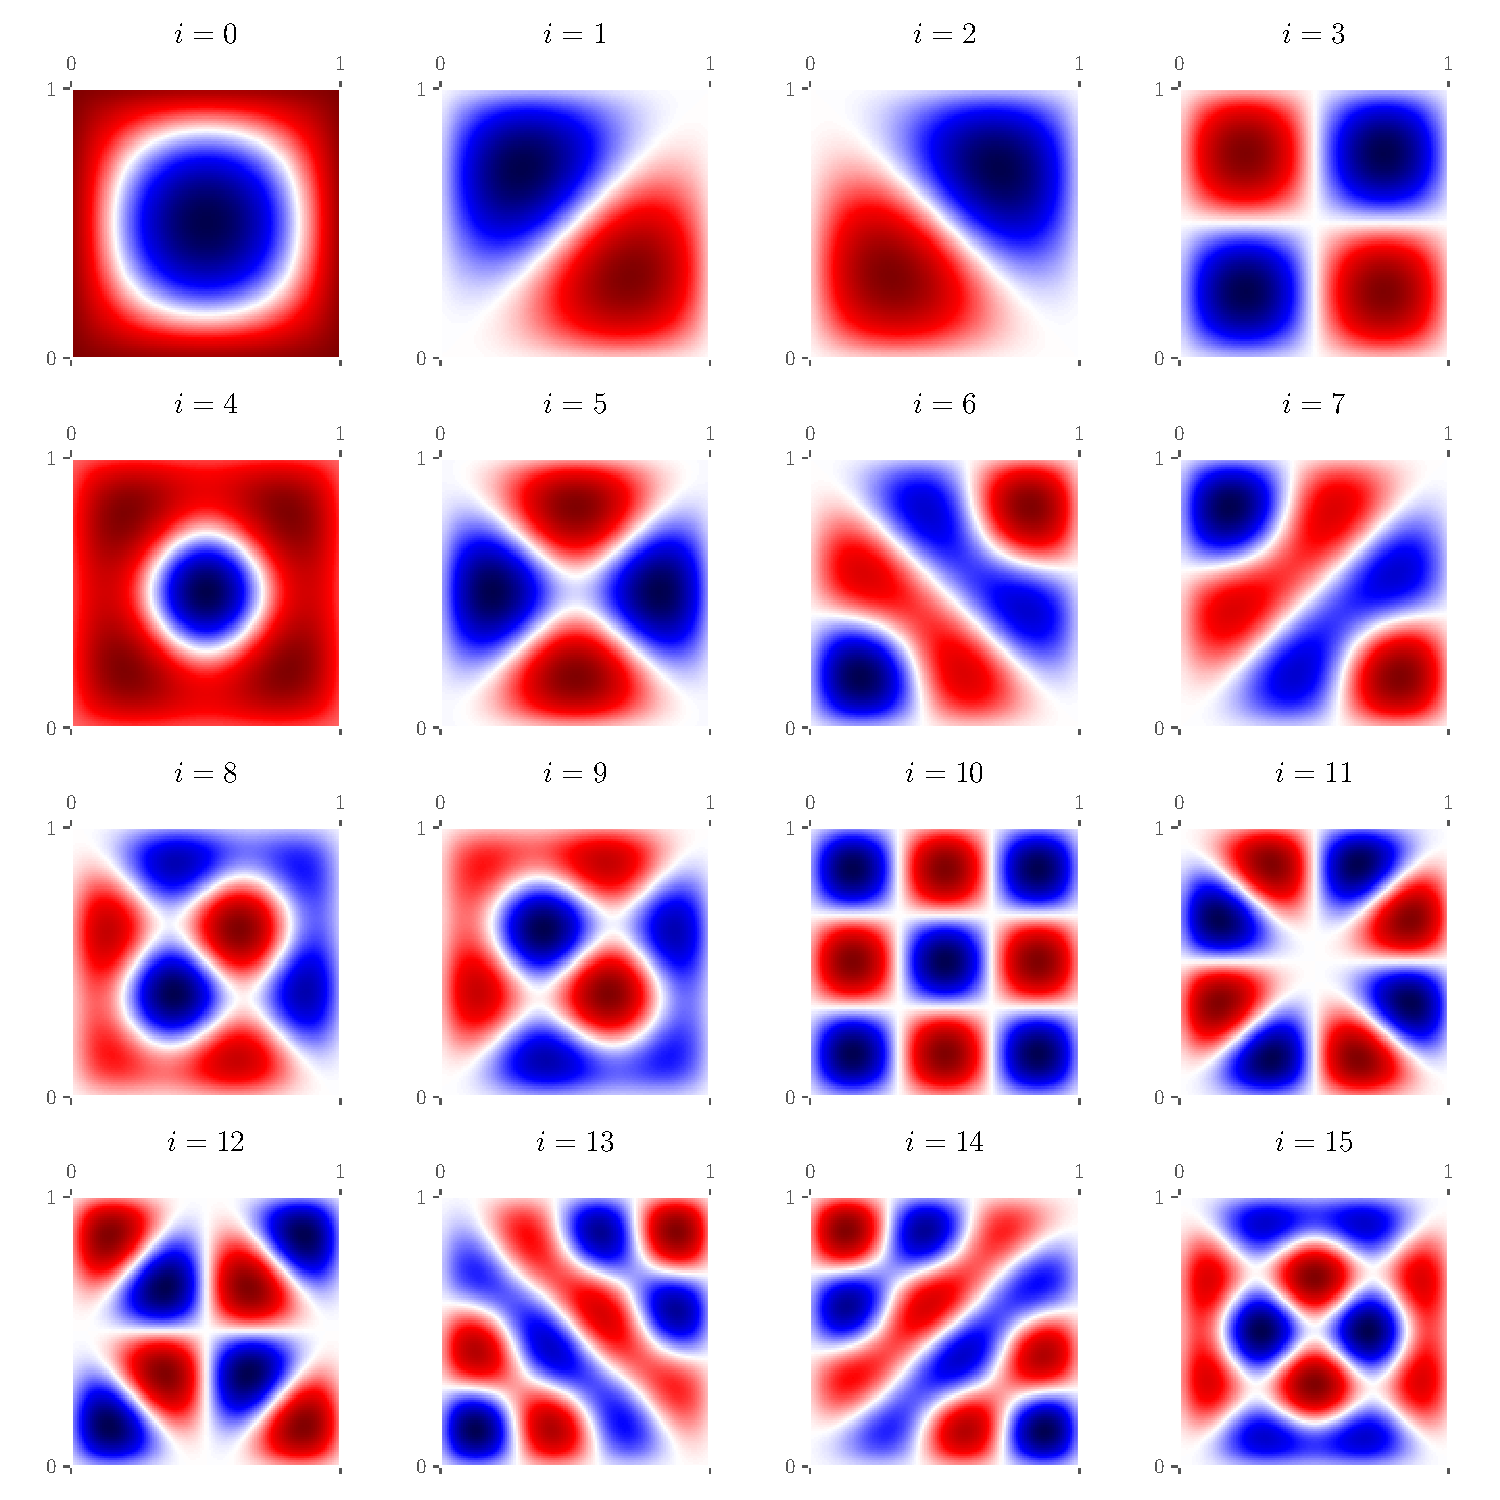
\includegraphics[width=0.7\textwidth]{../old/1-0-nihajni_nacini.pdf}
\end{center}
Če uporabimo metodo iz modula \texttt{scipy.sparse}, dobimo precej podobno sliko:
\begin{center}
    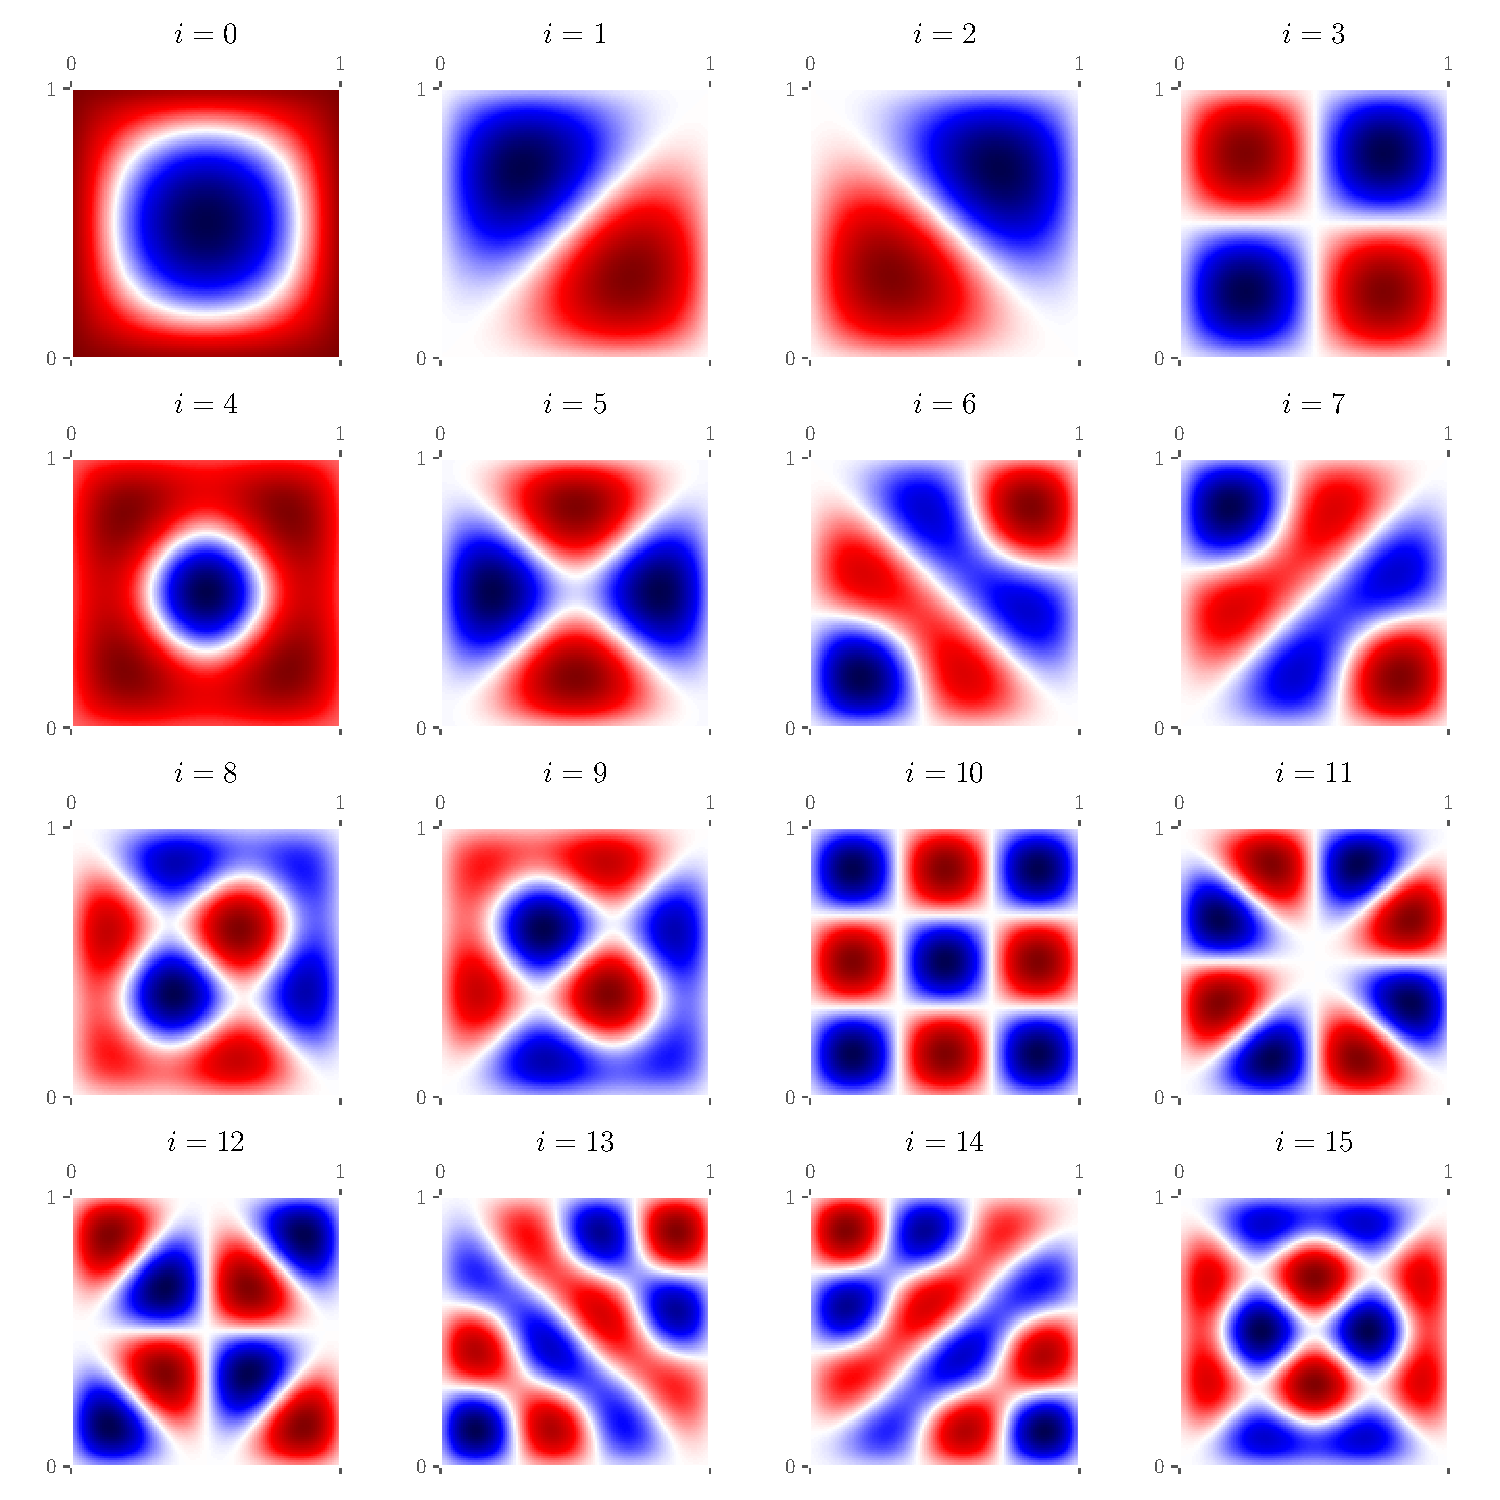
\includegraphics[width=0.7\textwidth]{../old/1-0-nihajni_nacini_sparse.pdf}
\end{center}
Nadaljeval sem z implementacijo potenčne metode. Sprva mi je nekaj težav predstavljala normalizacija lastnih vektorjev, a mi je kasneje uspelo:

\begin{center}
    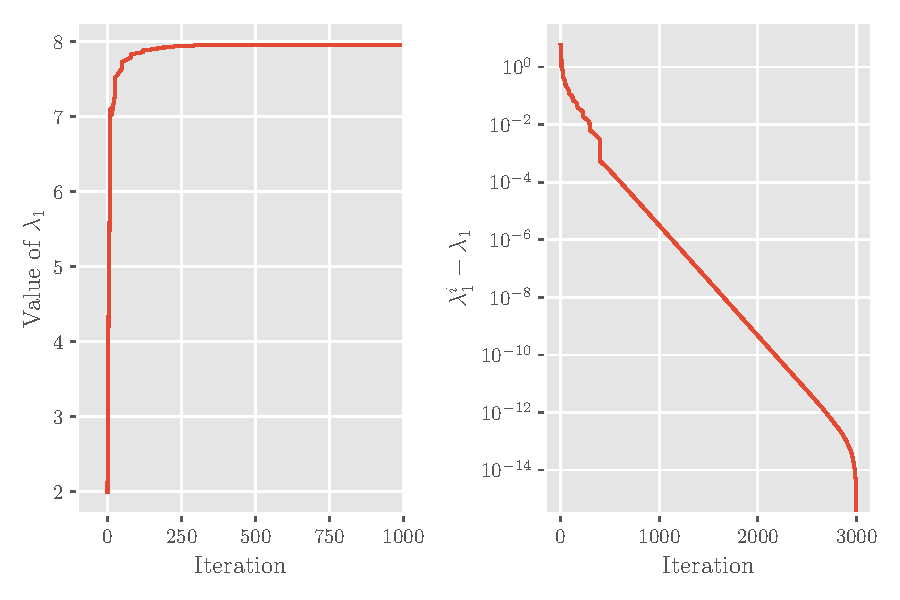
\includegraphics[width=0.8\textwidth]{../old/1-0-powermethod.pdf}
\end{center}

Naslednji korak je nadgradnja metode za konvergenco k poljubni lastni vrednosti. Opazim, da zaradi iskanja inverza matrike $A - \sigma I$ potrebujem mnogo več časa za enako število iteracij. Optimizacija z knjižnjico \texttt{numba.jit} ni uspela.  Pri generaciji spodnje slike sem uporabil začetni približek $\lambda = 8$ in dosegel isto lastno vrednost kot prej. Poleg potrebe po invertiranju matrike vsako iteracijo algoritem dodatno podaljša tudi dejstvo, da je $\mathcal{O}$ metode po \cite{wiki} enak
\[\left| \frac{\sigma - \lambda_{\text{iskana}}}{\lambda_{\text{ naslednja najbližja}} - \lambda_{\text{iskana}}} \right|\]

\begin{center}
    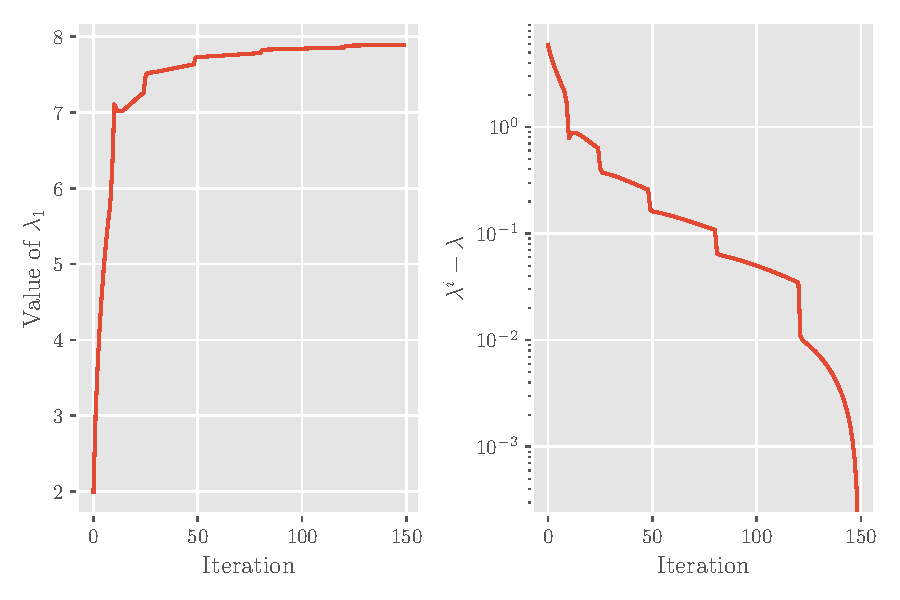
\includegraphics[width=0.8\textwidth]{../old/1-0-inverse_powermethod.pdf}
\end{center}

Če inverzno potenčno metodo uporabim na razponu od 0 do maksimalne lastne vrednosti, dobim spodnjo sliko, ki nakazuje, da metoda ne deluje, kot bi si želeli.
\begin{center}
    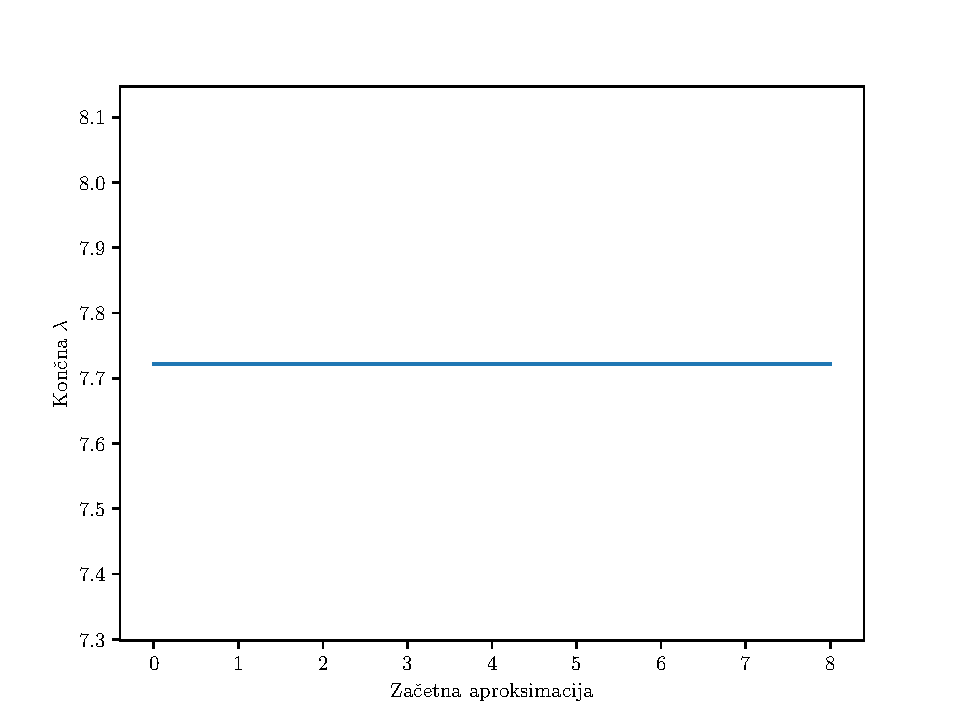
\includegraphics[width=0.7\textwidth]{../old/1-0-inverse_powermethod_sweep.pdf}
\end{center}
V nadaljevanju sem zgeneriral zahtevano figuro:
\begin{center}
    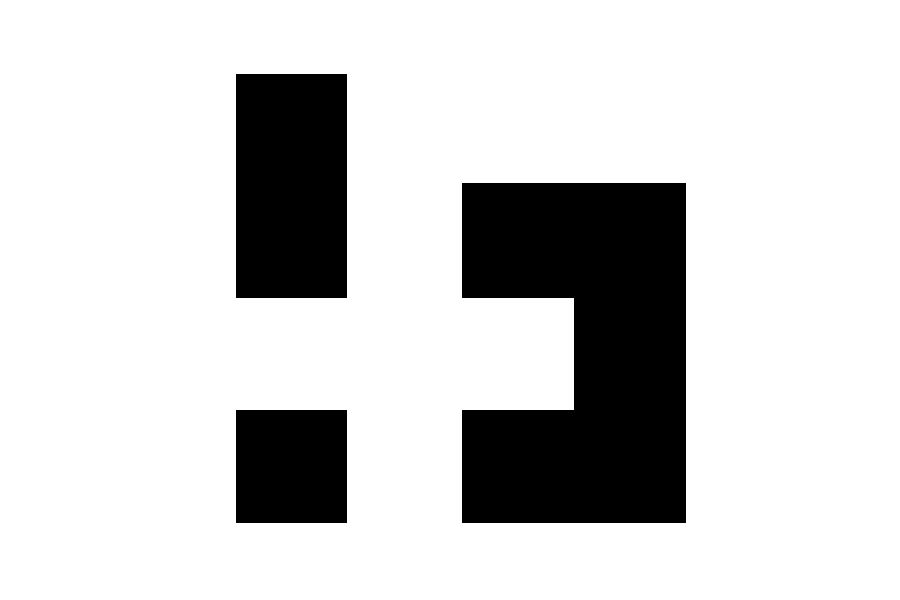
\includegraphics[width=0.5\textwidth]{../old/1-figura.pdf}
\end{center}

Če dobljeno gostotno matriko $\rho(x,y)$ preoblikujemo v diagonalno matriko, jo lahko uporabimo v metodi \texttt{scipy.linalg.eigh} in izračunamo lastne vrednosti in lastne vektorje kot poprej:
\begin{center}
    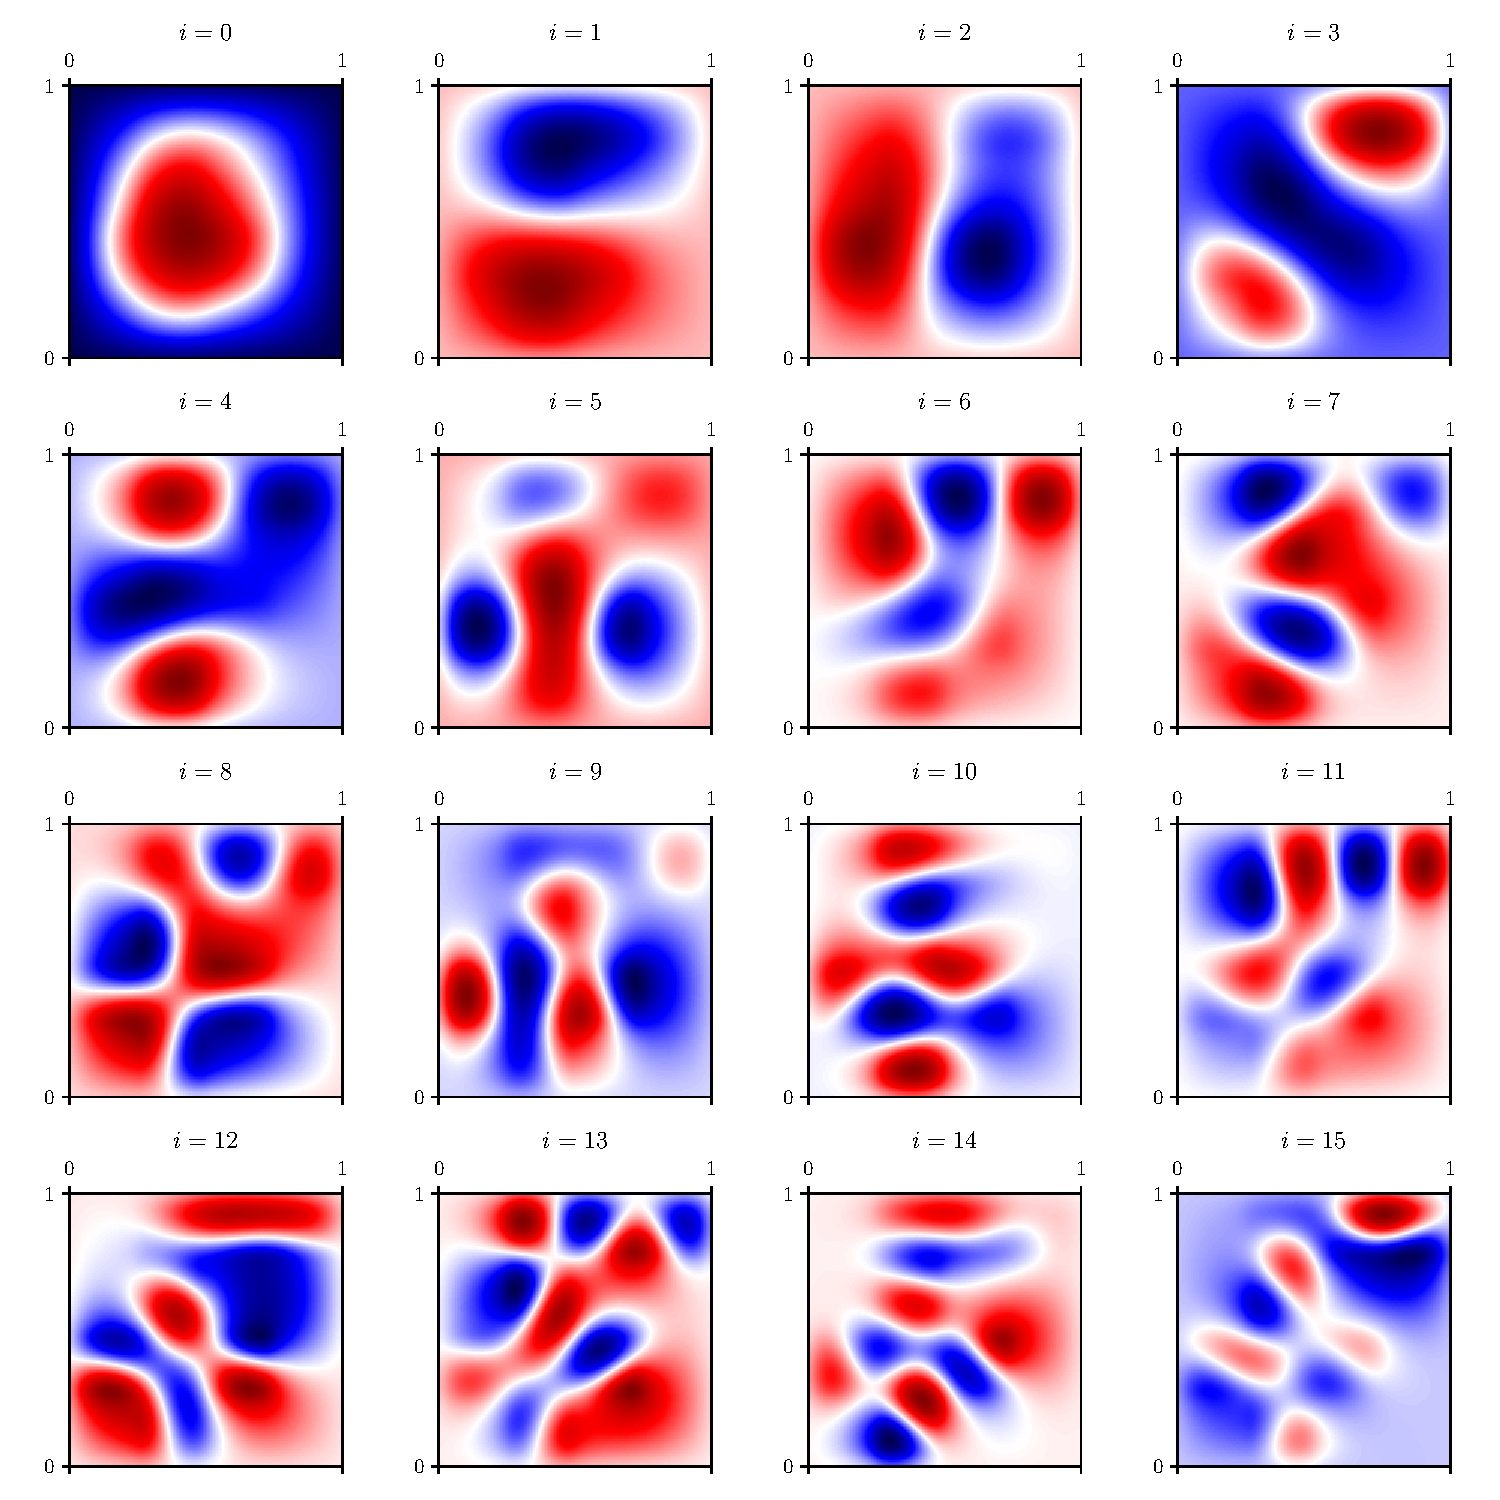
\includegraphics[width=\textwidth]{../old/1-1-nihajni_nacini.pdf}
\end{center}
Prikazujem prvih 16 nihajnih načinov, uporabljeni gostoti sta 1 in 10, osenčena območja so tako manj gosta. Če gostoti zamenjam, dobim naslednjo sliko.
\begin{center}
    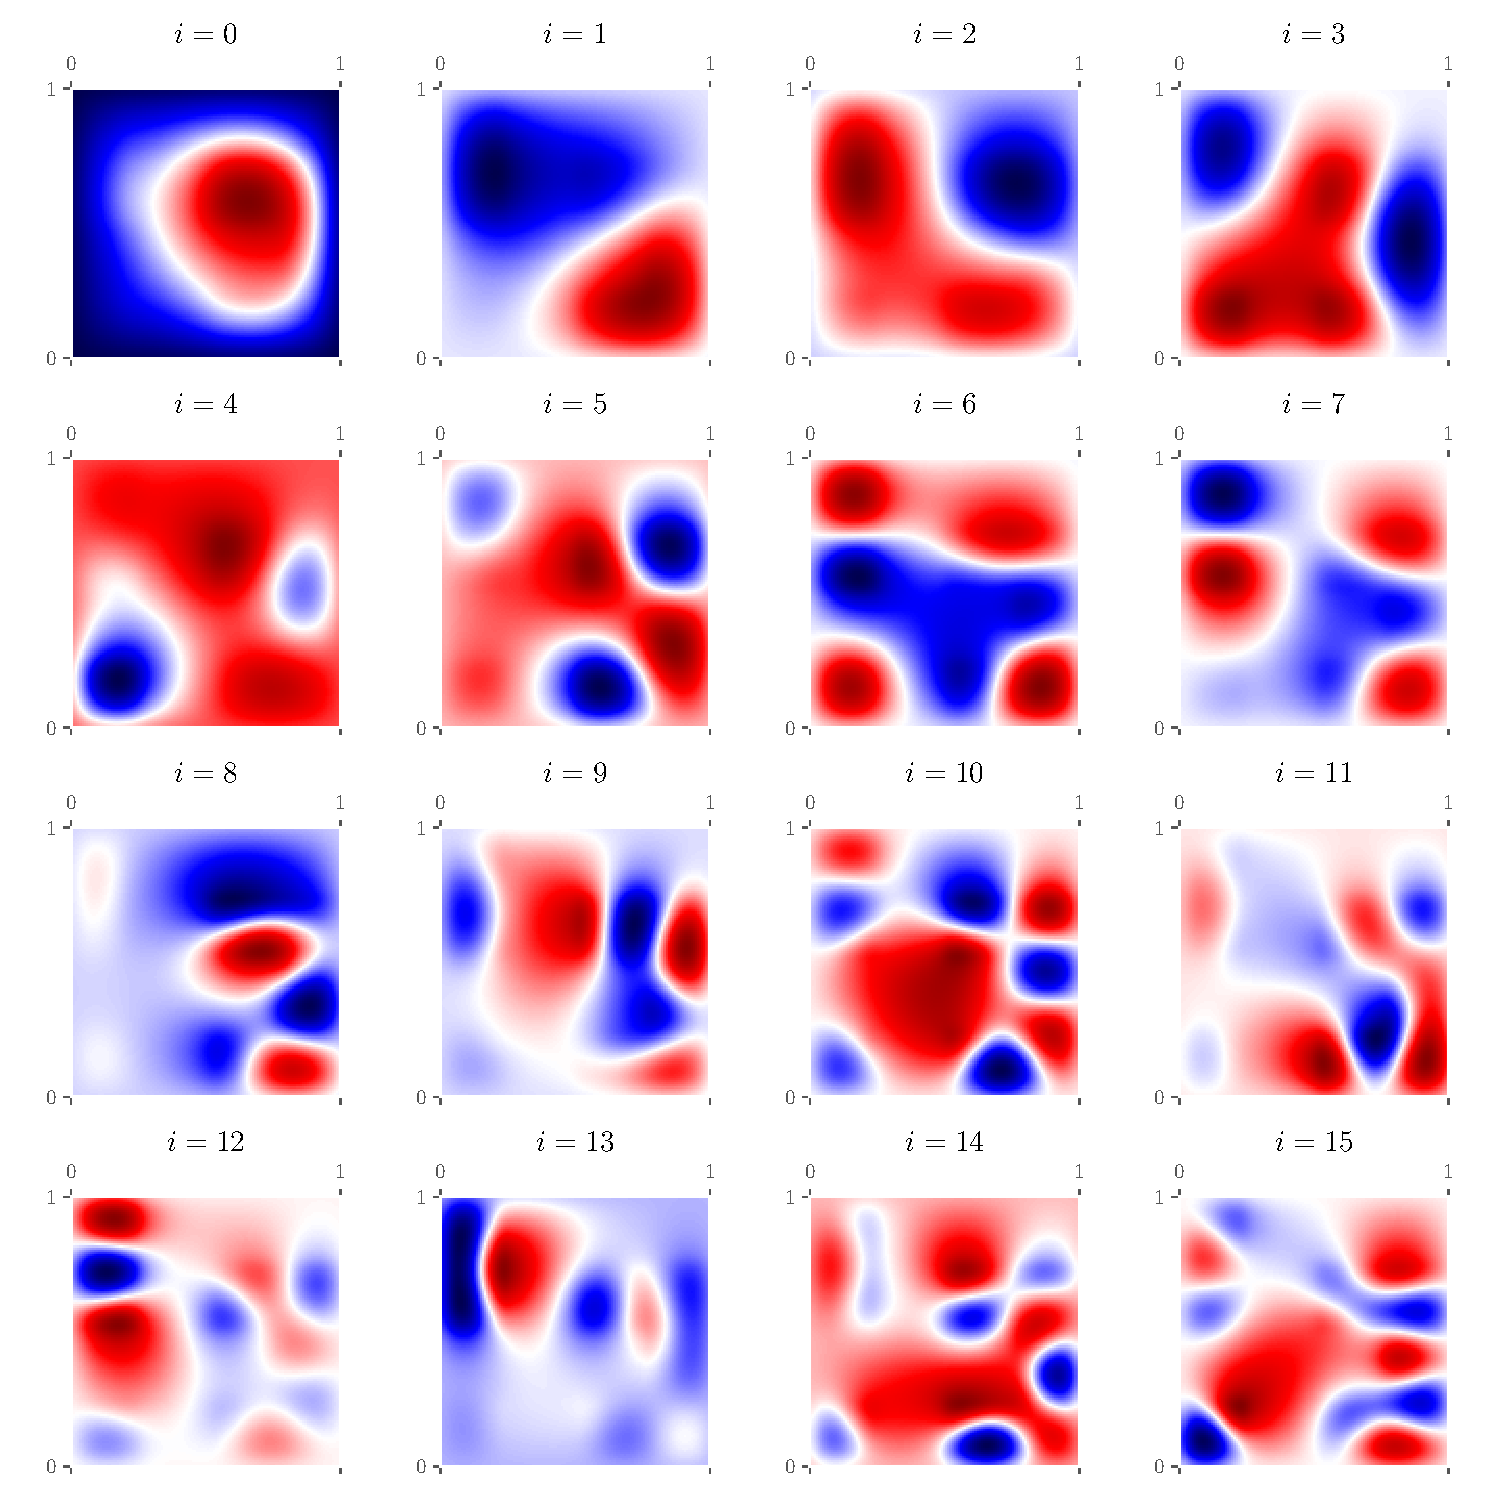
\includegraphics[width=\textwidth]{../old/1-1-nihajni_nacini_inverted.pdf}
\end{center}
Poglejmo si še spekter obeh obtežitev, začenši z najnižjimi 16 lastnimi vrednostmi.
\begin{center}
    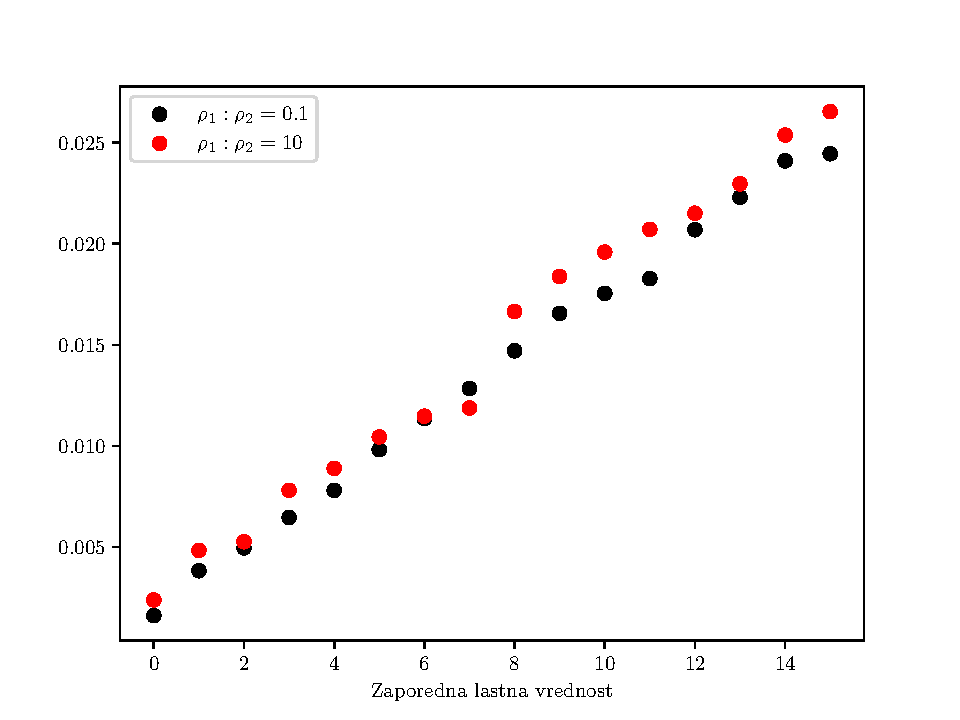
\includegraphics[width=\textwidth]{../old/1-1-spekter-zoom_both.pdf}
\end{center}
Če pogledamo celoten spekter obeh obtežitev, dobimo spodnjo sliko.
\begin{center}
    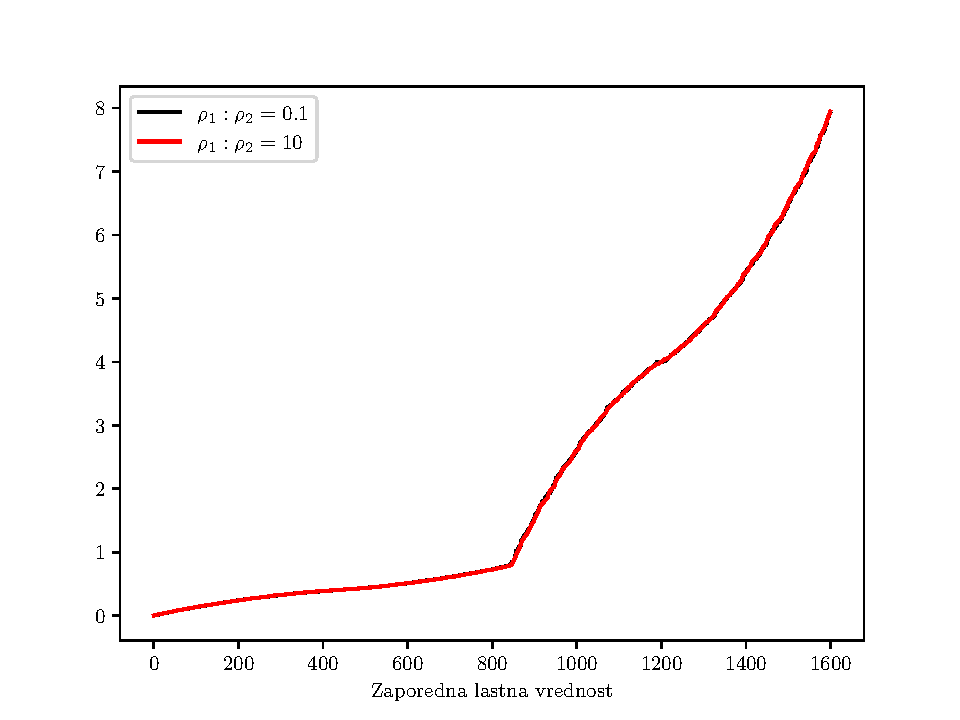
\includegraphics[width=\textwidth]{../old/1-1-spekter_both.pdf}
\end{center}
Očitno je, da pride nekje na polovici do diskontinuitete, zato sem si ta prehod pogledal pobližje na še bolj ekstremnem razmerju gostot 1000:1. Najnižja lastna nihanja izgledajo presenetljivo podobna vsem ostalim:
\begin{center}
    \centering
        \begin{minipage}{0.45\textwidth}
        \centering
    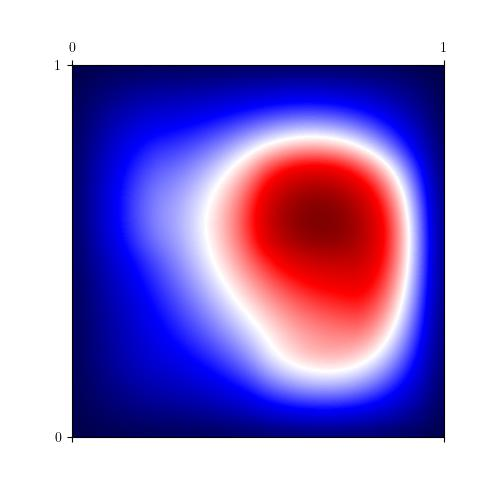
\includegraphics[width=\textwidth]{../old/1-1-eigenmode-0.jpg}
    Prvi nihajni način za razmerje gostot 1000:1.
    \end{minipage}\hfill
    \begin{minipage}{0.45\textwidth}
        \centering
        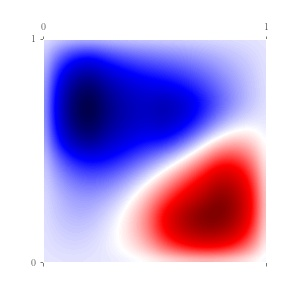
\includegraphics[width=1\textwidth]{../old/1-1-eigenmode-1.jpg}
        Drugi nihajni način za isto opno.
    \end{minipage}
    \begin{minipage}{0.45\textwidth}
        \centering
    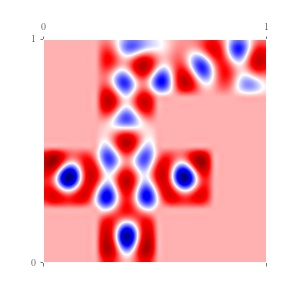
\includegraphics[width=\textwidth]{../old/1-1-eigenmode-849.jpg}
    850. nihajni način za razmerje gostot 1000:1.
    \end{minipage}\hfill
    \begin{minipage}{0.45\textwidth}
        \centering
        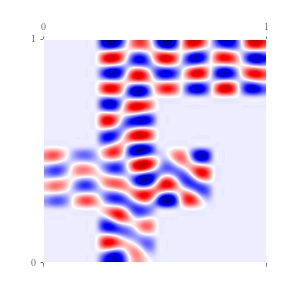
\includegraphics[width=1\textwidth]{../old/1-1-eigenmode-900.jpg}
        901. nihajni način za isto opno.
    \end{minipage}
\end{center}
Postuliram, da zaradi diskontinuitete v spektru pride zaradi kvalitativno različnih nihanj; če prej celotna opna niha kot celota, po neki kritični lastni vrednosti težji deli opne obmirujejo, nihanje pa se z venomer večjimi valovnimi števili razvije v lažjem delu.

